%%% LaTeX Template: Article/Thesis/etc. with colored headings and special fonts
%%%
%%% Source: http://www.howtotex.com/
%%% Feel free to distribute this template, but please keep to referal to http://www.howtotex.com/ here.
%%% February 2011
%%%
%%% Modified January 2016 by CDM

%%%  Preamble
\documentclass[11pt,letterpaper]{article}
\usepackage[margin=1.0in]{geometry}
\usepackage[T1]{fontenc}
\usepackage[bitstream-charter]{mathdesign}
\usepackage[latin1]{inputenc}					
\usepackage{amsmath}						
\usepackage{xcolor}
\usepackage{cite}
\usepackage{hyphenat}
\usepackage{graphicx}
\usepackage{float}
\usepackage{subfigure}
\usepackage{sectsty}
\usepackage[compact]{titlesec} 
\usepackage[tablegrid]{vhistory}
\usepackage{pbox}
\allsectionsfont{\color{accentcolor}\scshape\selectfont}

%%% Definitions
\definecolor{accentcolor}{rgb}{0.0,0.0,0.5} 
\newcommand{\teamname}{Team Demeter}
\newcommand{\productname}{DemeBot}
\newcommand{\coursename}{CSE 4316: Senior Design II}
\newcommand{\semester}{Spring 2017}
\newcommand{\docname}{Detailed Design Specification}
\newcommand{\department}{Department of Computer Science \& Engineering}
\newcommand{\university}{The University of Texas at Arlington}
\newcommand{\authors}{Arun Kalahasti \\ Bipin Ghimire \\ Saman Shrestha \\ Santosh Pradhan \\ Travis Matthews}

%%% Headers and footers
\usepackage{fancyhdr}
	\pagestyle{fancy}						% Enabling the custom headers/footers
\usepackage{lastpage}	
	% Header (empty)
	\lhead{}
	\chead{}
	\rhead{}
	% Footer
	\lfoot{\footnotesize \teamname \ - \semester}
	\cfoot{}
	\rfoot{\footnotesize page \thepage\ of \pageref{LastPage}}	% "Page 1 of 2"
	\renewcommand{\headrulewidth}{0.0pt}
	\renewcommand{\footrulewidth}{0.4pt}

%%% Change the abstract environment
\usepackage[runin]{abstract}			% runin option for a run-in title
%\setlength\absleftindent{30pt}			% left margin
%\setlength\absrightindent{30pt}		% right margin
\abslabeldelim{\quad}	
\setlength{\abstitleskip}{-10pt}
\renewcommand{\abstractname}{}
\renewcommand{\abstracttextfont}{\color{accentcolor} \small \slshape}	% slanted text

%%% Start of the document
\begin{document}

%%% Cover sheet
{\centering \huge \color{accentcolor} \sc \textbf{\department \\ \university} \par}
\vspace{1 in}
{\centering \huge \color{accentcolor} \sc \textbf{\docname \\ \coursename \\ \semester} \par}
\vspace{0.5 in}
\begin{figure}[h!]
	\centering
   	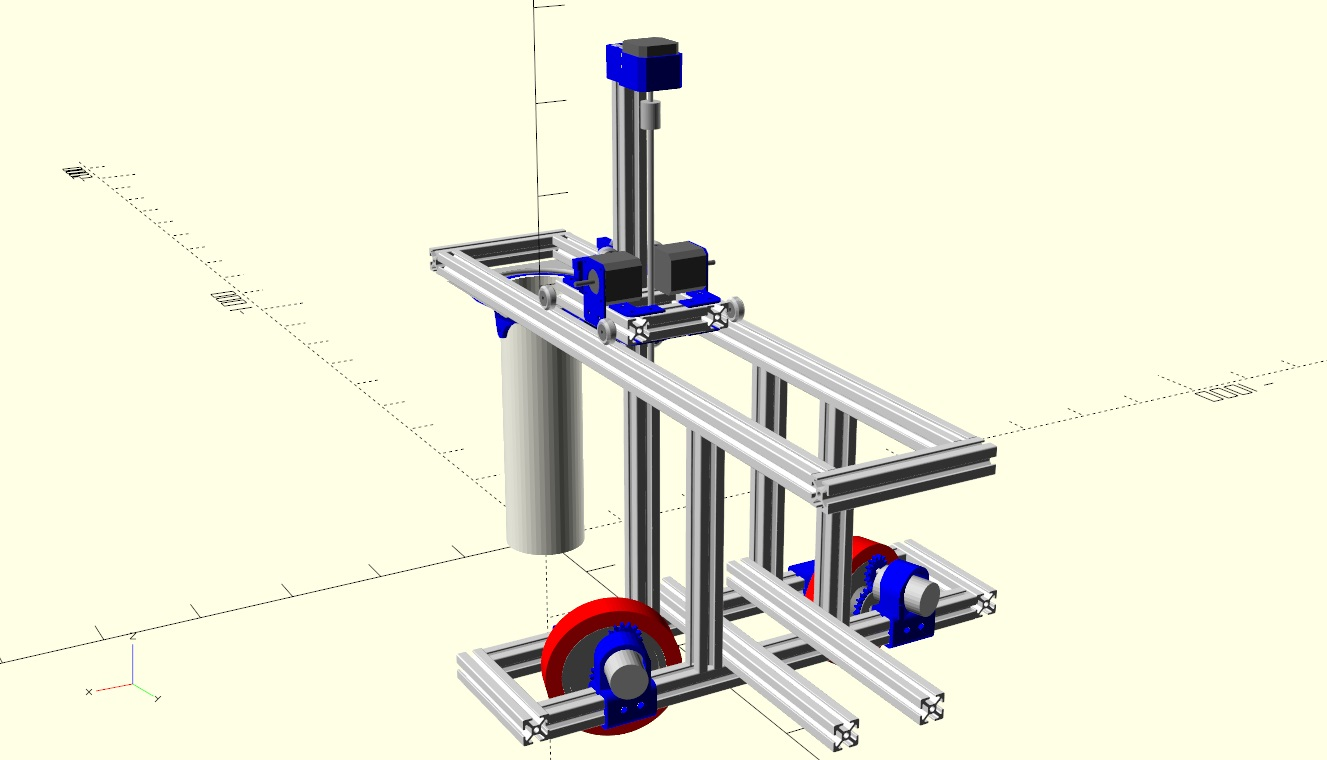
\includegraphics[width=0.60\textwidth]{images/detailed}
\end{figure}
\vspace{0.5 in}
{\centering \huge \color{accentcolor} \sc \textbf{\teamname \\ \productname} \par}
\vspace{0.5 in}
{\centering \large \sc \textbf{\authors} \par}
\newpage


%\vspace{1 in}
%\centerline{January 13th, 2012}
%\newpage

%%% Revision History
\begin{versionhistory}
  	\vhEntry{1.0}{11.14.2016}{AK}{official release}
\end{versionhistory}
\newpage

%%% Table of contents
\setcounter{tocdepth}{2}
\tableofcontents
\newpage

%%% List of figures and tables (optional)
\listoffigures
\listoftables
\newpage

%%% Document sections
\section{Introduction}
Polar FarmBot is a CNC robot that will automate the agricultural growing process. It will be able to plant seeds, water plants, measure soil conditions, and remove weeds. The system will not be able to harvest plants nor remove pests from the plants. It will be stationed in a backyard and will be used to grow various fruits and vegetables such as carrots, lettuce, watermelon, onions, and much more along with all kinds of spices and herbs.

Polar FarmBot will have a central pole in which an arm pivots around. The arm will extend outward from the central pole at variable lengths depending on the size specified by the consumer. At the end of the arm there will be a support that extends downward to a set of wheels that allow the arm to move in a circular direction around the central pole. Along the arm there will be a gantry system that will be powered by a motor to move horizontally back and forward on the arm. The gantry will also have a separate motor that will power a separate arm that moves up and down in the vertical direction. Attached to the rod will be the seeder, water pump, and soil monitor tool assembly. Cables and connectors will be routed through the arm, down the central pole, and back out to a control box located just outside the gardening plot. Within the control box, there will be a motor driver and raspberry pi. The motor driver will power all the motors and sensors on the gantry. The raspberry pi will connect to the internet that will allow for a web based user interface to interact with the system. The control box will also house a power supply that will power all the motors, sensors, motor driver, and raspberry pi. There will also be connectors for the vacuum for picking up seeds and also a connector for water that will allow the robot the ability to water plants.

The robot will also connect back to a computer that will have a web interface for users to interact with the robot. From this interface a user will be able to layout a plot, monitor overall plant growth and soil conditions, and see whether or not the plants are ready for harvesting. To go along with the web interface, there will be a companion application developed for android. This app will have all the same functionality as the web app just on a mobile platform. Polar FarmBot will have multiple cameras attached to it to allow monitoring progress remotely.
\newpage
\section{System Overview}
PolarFarmBot will be a CNC robot that will automate the agricultural process. The robot will pivot around a central pole and have a tool assembly that will moved in and out along the arm of the robot.
PolarFarmBot will plant seeds, water plants, measure soil moisture levels, calculate soil pH levels, and remove weeds.
The robot will connect back to a computer that will have a web interface for users to interact with the robot. From this interface a user will be able to layout a plot, monitor overall plant growth and soil conditions, and see whether or not the plants are ready for harvesting.
To go along with the web interface, there will be a companion application developed for android. This app will have all the same functionality as the web app just on a mobile platform.
PolarFarmBot will have multiple cameras attached to it to allow monitoring progress remotely.


\begin{figure}[h!]
    \centering
    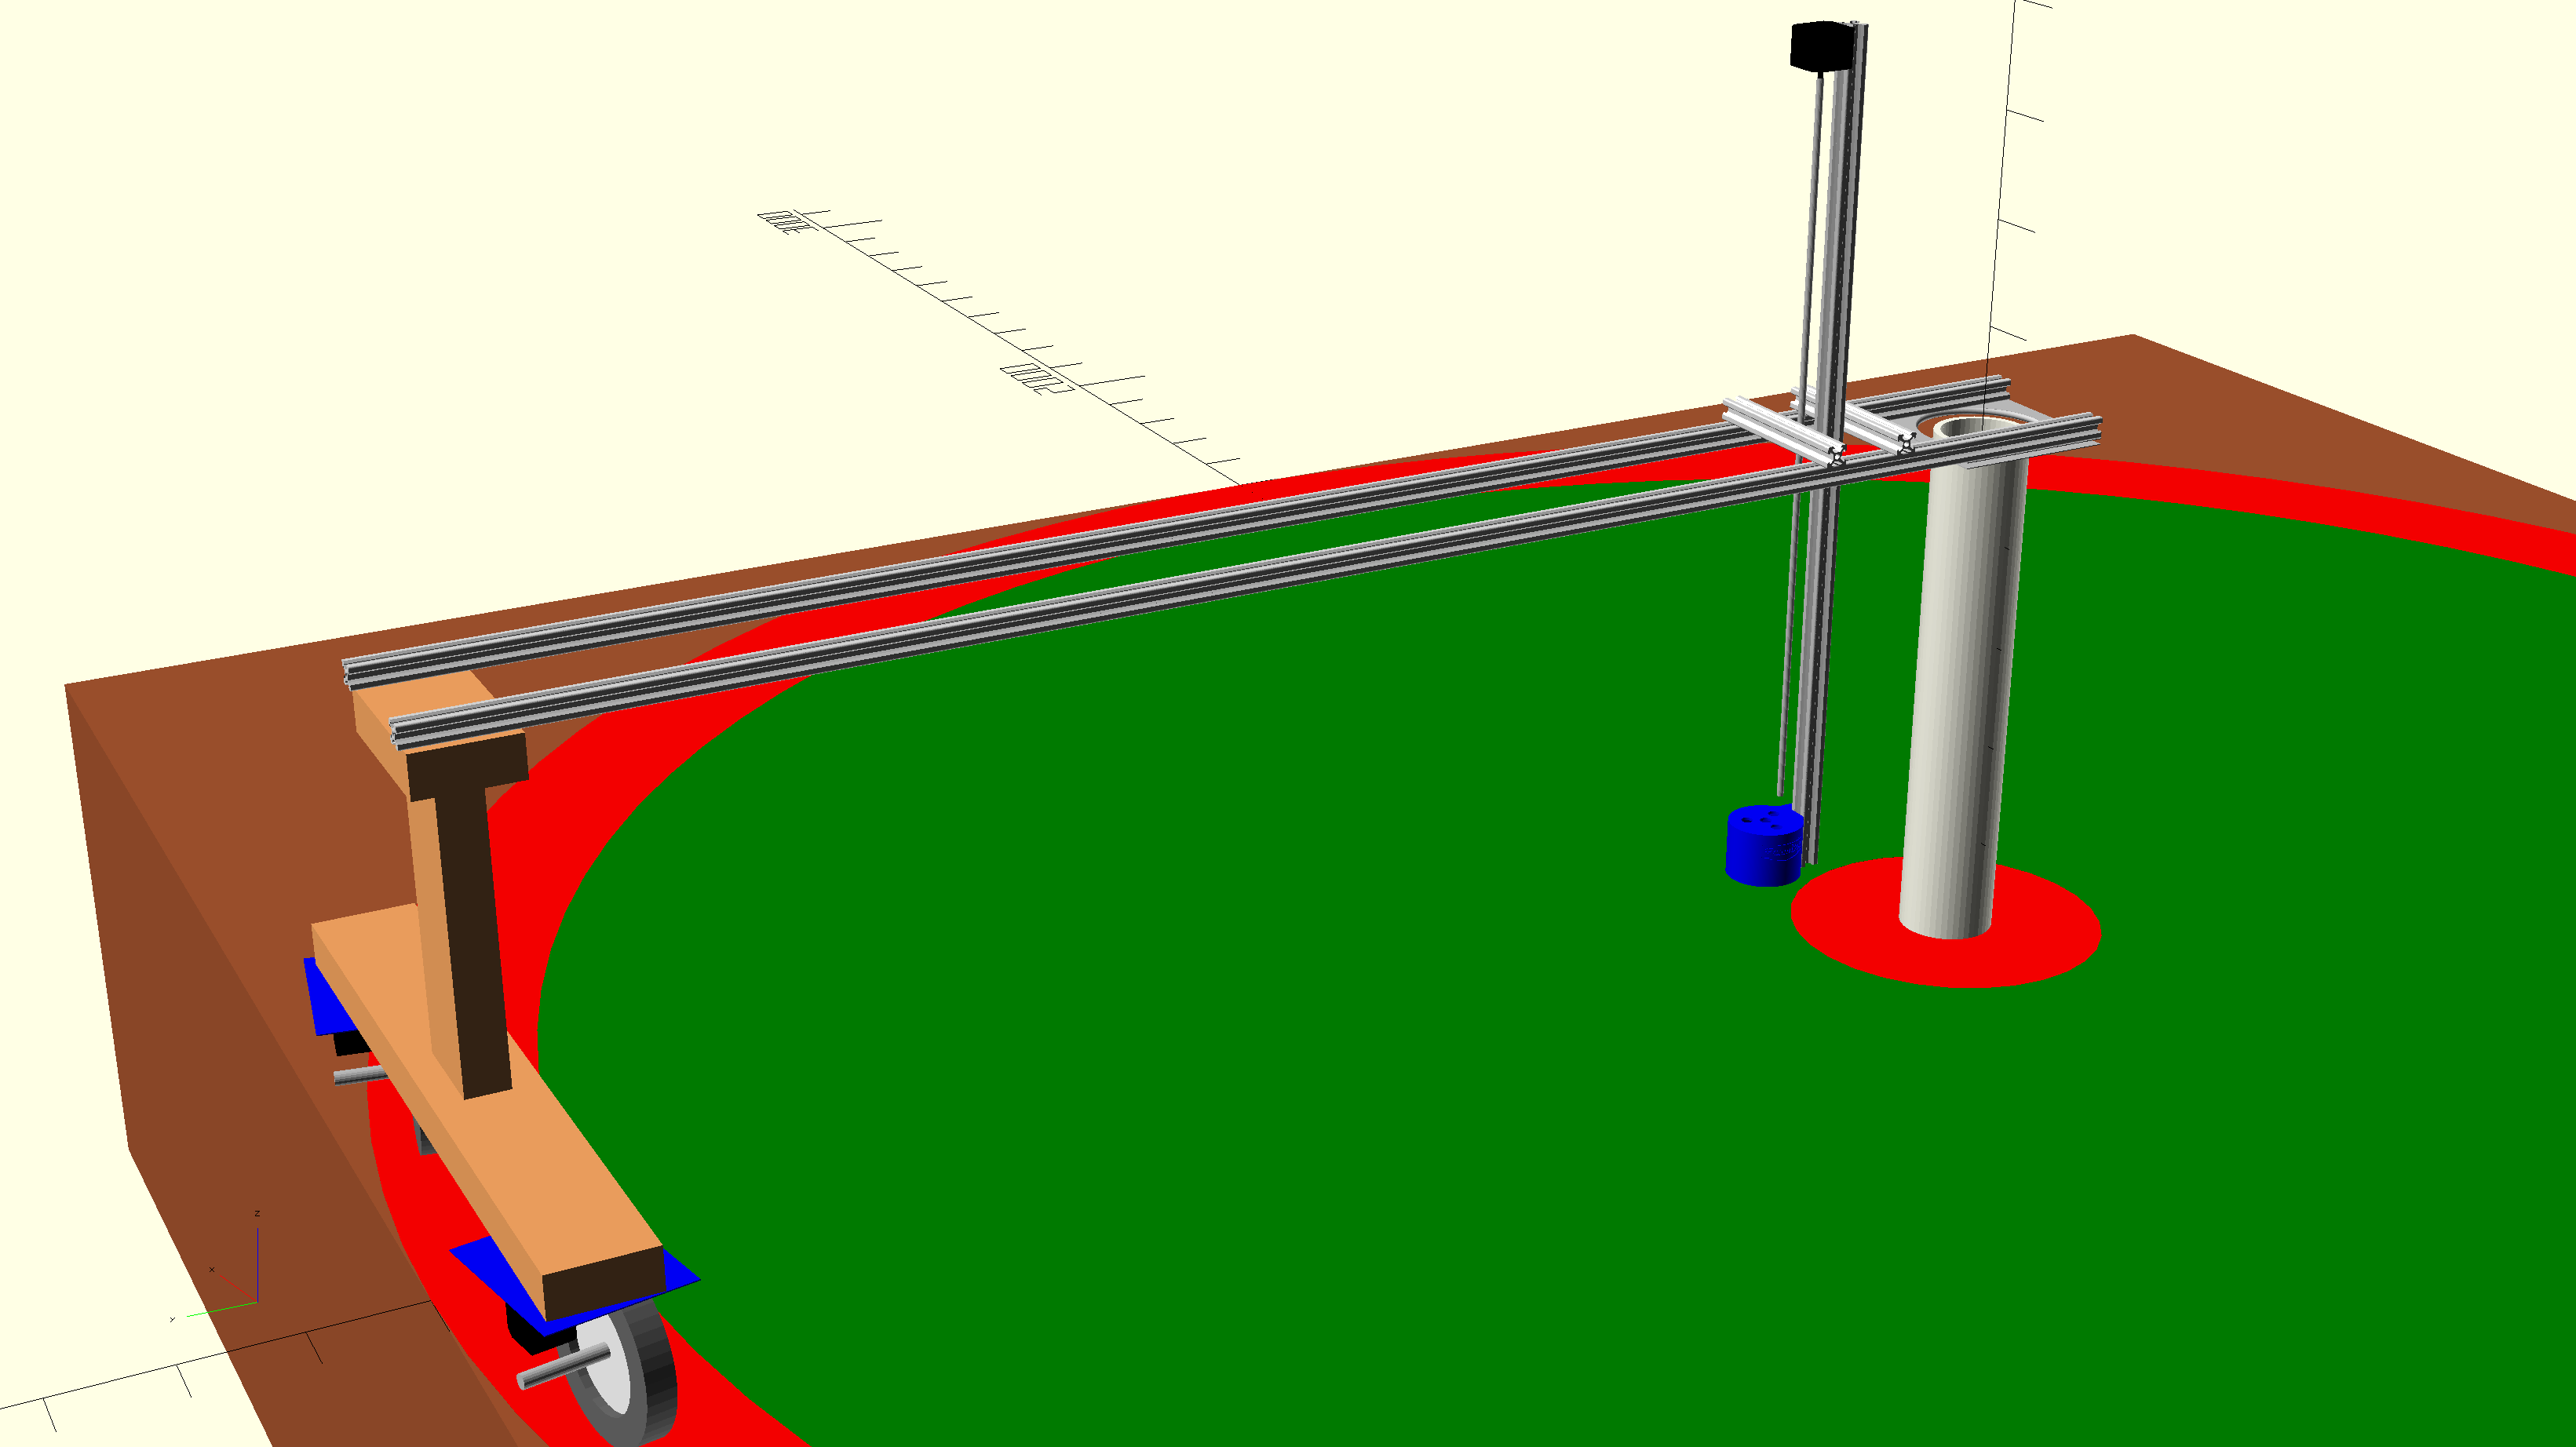
\includegraphics[width=0.75\textwidth]{images/arm-closeup}
    \caption{Deatailed view of mock-up arm design}
\end{figure}
\newpage
\section{Subsystem Definitions \& Data Flow}
The data flow in the Farm Bot architectural design starts from the I/O sub layer in the Web Client layer. The user gives the input through the web interface and it reaches to the Web API Layer. In Web API layer, the data flows to the core logic layer through web gateway. The data will also flow between the core and the User/Access Authentication layers to validate the user access. The core will be able to access database as per the request from user through database interface. In the Core Logic Layer, G-Code Generator generates the G-Code in the form of processes which are lined up by the Scheduler based on their priority in the command pipeline. Then, those processes are transmitted to the Motor Control Layer through the Serial Command Interface and are executed in the G-code Processor. These processed signals help motor to move to the precise coordinates.   

\begin{figure}[h!]
	\centering
 	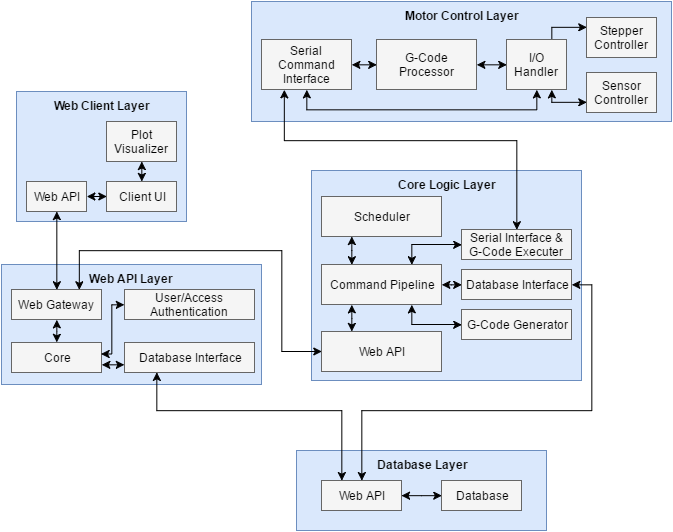
\includegraphics[width=\textwidth]{images/data_flow}
 \caption{A simple data flow diagram}
\end{figure}

\newpage
\section{Core Logic Layer Subsystems}
The Core Logic Layer subsystems are centered around planning and executing the main actions needed by the machine. 

\subsection{Command Pipeline}
The Command Pipeline is a ordered que of actions which are known to need execution. Each action is read off the top of the list and executed at an indicated time. The command pipeline must also assign an action to the appropriate system for execution.

\begin{figure}[h!]
	\centering
 	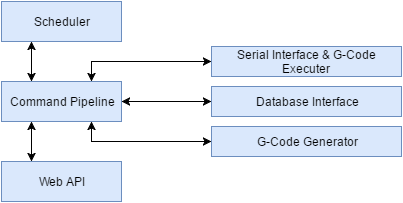
\includegraphics[width=0.60\textwidth]{images/core_logic_layer}
 \caption{Example subsystem description diagram}
\end{figure}

\subsubsection{Assumptions}
The command pipeline assumes that the other system components are always available to execute commands. 

\subsubsection{Responsibilities}
The command pipeline must accurately maintain the order of execution for its tasks.

\subsubsection{Subsystem Interfaces}
The command pipeline must be able to interface with all the other systems it executes commands for. The primary interface for these transactions is through a html web API. 

\begin {table}[H]
\caption {Subsystem interfaces} 
\begin{center}
    \begin{tabular}{ | p{1cm} | p{6cm} | p{3cm} | p{3cm} |}
    \hline
    ID & Description & Inputs & Outputs \\ \hline
    \#01 & Scheduler bus & \pbox{3cm}{Upcomming task events} & \pbox{3cm}{Future Actions needed}  \\ \hline
    \#02 & Serial Pipeline & \pbox{3cm}{Serial Data} & \pbox{3cm}{Serial Commands}  \\ \hline
    \#03 & G-Code interface & \pbox{3cm}{Serial Data} & \pbox{3cm}{Serial Commands}  \\ \hline
    \end{tabular}
\end{center}
\end{table}

\subsection{Scheduler}
The Scheduler subsystem is built to store requested command events as well as request their timely execution by the command pipeline

\subsubsection{Assumptions}
The scheduler is assumed to be constantly running. 

\subsubsection{Responsibilities}
The primary purpose of the scheduler was to ensure commands have been executed in a timely manner. This necessitates an internal time tracking system to ensure commands are being executed when they are scheduled to.

\subsubsection{Subsystem Interfaces}
The scheduler subsystem only needs to interface directly with the command pipeline. It must be able to send and recieve full command instructions as used by the command pipeline.

\begin {table}[H]
\caption {Subsystem interfaces} 
\begin{center}
    \begin{tabular}{ | p{1cm} | p{6cm} | p{3cm} | p{3cm} |}
    \hline
    ID & Description & Inputs & Outputs \\ \hline
    \#01 & Scheduler bus & \pbox{3cm}{Upcoming  task events} & \pbox{3cm}{Future Actions needed}  \\ \hline
    \end{tabular}
\end{center}
\end{table}

\subsection{Web API}
The Web API subsystem is to allow interfacing to the rest of the FarmBot systems.

\subsubsection{Assumptions}
The Web API subsystem is assumed to not need user authentication for security. 

\subsubsection{Responsibilities}
The Web API subsystem must listen for input from other layers within the FarmBot architecture. If the input is not provided in a sensible manner, it must be transformed in the subsystem. 

\subsubsection{Subsystem Interfaces}
The Web API subsystem provides an unsecured html interface. 

\begin {table}[H]
\caption {Subsystem interfaces} 
\begin{center}
    \begin{tabular}{ | p{1cm} | p{6cm} | p{3cm} | p{3cm} |}
    \hline
    ID & Description & Inputs & Outputs \\ \hline
    \#01 & HTML & \pbox{3cm}{html requests} & \pbox{3cm}{html responses}  \\ \hline
    \end{tabular}
\end{center}
\end{table}

\subsection{Database Interface}
The Database Interface subsystem allows data transactions to the central database. 

\subsubsection{Assumptions}
The data passing though the database interface is assumed to be in the final form required before storing. The Database Layer may not always be available.

\subsubsection{Responsibilities}
The database interface must attempt to send data to the Database Layer of the FarmBot. Data which cannot immediately be pushed to the data layer will be buffered within the subsystem until a timeout or the Database Layer accepts the data.

\subsubsection{Subsystem Interfaces}
The Database interface only communicates to the command pipeline subsystem and the database layer API. 

\begin {table}[H]
\caption {Subsystem interfaces} 
\begin{center}
    \begin{tabular}{ | p{1cm} | p{6cm} | p{3cm} | p{3cm} |}
    \hline
    ID & Description & Inputs & Outputs \\ \hline
    \#01 & Command Pipeline & \pbox{3cm}{Data store requests} & \pbox{3cm}{responses}  \\ \hline
    \end{tabular}
\end{center}
\end{table}

\subsection{G-Code Generator}
The G-Code generator subsystem is the software element which converts command actions in the pipeline into executable machine movement code.  

\subsubsection{Assumptions}
The development of this subsystem assumes that complex actions can be consistently digested into a series of motor control actions. 

\subsubsection{Responsibilities}
The G-Code generator will be responsible for creating all motor control actions. 

\subsubsection{Subsystem Interfaces}
The G-Code Generator only communicates to the command pipeline subsystem.

\begin {table}[H]
\caption {Subsystem interfaces} 
\begin{center}
    \begin{tabular}{ | p{1cm} | p{6cm} | p{3cm} | p{3cm} |}
    \hline
    ID & Description & Inputs & Outputs \\ \hline
    \#01 & Command Pipeline & \pbox{3cm}{Actions} & \pbox{3cm}{G-Code Commands}  \\ \hline
    \end{tabular}
\end{center}
\end{table}

\subsection{Serial Interface}
The serial interface connects the core logic layer to the motor control layer.

\subsubsection{Assumptions}
We are assuming the motor control layer requires no input from the rest of the systems beyond coordinate actions. We are also assuming the motor control layer acknowledges receiving all instructions and if no response is received by the motor control layer the instruction was unable to be executed.

\subsubsection{Responsibilities}
The Serial Interface is responsible for parsing action in the command pipeline sending them to the motor control layer. 

\subsubsection{Subsystem Interfaces}
The Serial Interface only communicates to the command pipeline subsystem and the motor control layer.

\begin {table}[H]
\caption {Subsystem interfaces} 
\begin{center}
    \begin{tabular}{ | p{1cm} | p{6cm} | p{3cm} | p{3cm} |}
    \hline
    ID & Description & Inputs & Outputs \\ \hline
    \#01 & Command Pipeline & \pbox{3cm}{G-Code Commands} & \pbox{3cm}{Serial Strings}  \\ \hline
    \end{tabular}
\end{center}
\end{table}
\newpage
\section{Motor Control Layer Subsystems}
The Motor Control Layer controls the machine frame and executes actions requested by the core logic layer. The commands will be sent through a serial interface in the G-Code syntax. The Motor Control Layer will parse these commands, translate them to the machine required machine configuration, and manipulate the motors on the frame to match. If the commands are sensor data requests the I/O handler will translate the raw sensor data into a string format and transmit it back across the serial interface.

\begin{figure}[h!]
	\centering
 	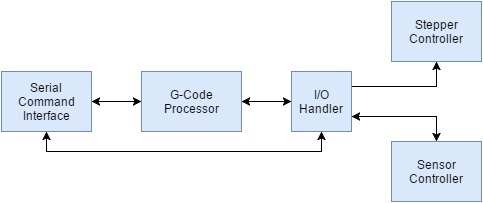
\includegraphics[width=0.60\textwidth]{images/motor_control_layer}
 \caption{Example subsystem description diagram}
\end{figure}

\subsection{Serial Command Interface}
Ther Serial Command Interface is the only method of communication available to the entire Motor Control Layer. This subsystem receives character input through a serial bus and must parse them into individual instructions. These instructions are then routed to the appropriate subsystem for execution. The interface will also build return statements and transmit them as requested by the other Motor Control Layer subsystems. 

\subsubsection{Assumptions}
The Serial Command Interface should not receive commands longer than the limiting buffer. Any commands which are longer than that will not be executed, returning an error through the Serial Command Interface to the control system. The control system is assumed to understand that a command was unable to be parsed and attempt to recover without further action from the Serial Command Interface.

\subsubsection{Responsibilities}
The Serial Command Interface is responsible for parsing all character input into parametrized commands for consumption by the appropriate subsystem. The interface must request a retransmit if there is an error in parsing the input or return a command acknowledged message if parsing was successful. When the Serial Control Interface sends a message to the Core Logic Layer it does not expect a result. 

\subsubsection{Subsystem Interfaces}

\begin {table}[H]
\caption {Subsystem interfaces} 
\begin{center}
    \begin{tabular}{ | p{1cm} | p{6cm} | p{3cm} | p{3cm} |}
    \hline
    ID & Description & Inputs & Outputs \\ \hline
    \#01 & Serial Bus Interface & \pbox{3cm}{characters over bus} & \pbox{3cm}{characters over bus}  \\ \hline
    \end{tabular}
\end{center}
\end{table}

\subsection{G-Code Processor}
The G-Code Processor processes Cartesian coordinate commands into polar configurations which can be used to control the machine. 

\subsubsection{Responsibilities}
This subsystem must intercept control commands which were sent using Cartesian coordinates and convert them to polar coordinates before passing them to the I/O Handler subsystem.  

\subsubsection{Subsystem Interfaces}

\begin {table}[H]
\caption {Subsystem interfaces} 
\begin{center}
    \begin{tabular}{ | p{1cm} | p{6cm} | p{3cm} | p{3cm} |}
    \hline
    ID & Description & Inputs & Outputs \\ \hline
    \#01 & Serial Command Interface & \pbox{3cm}{String array} & \pbox{3cm}{N/A}  \\ \hline
    \#02 & I/O Handler & \pbox{3cm}{N/A} & \pbox{3cm}{String array}  \\ \hline
    \end{tabular}
\end{center}
\end{table}

\subsection{I/O Handler}
The I/O Handler executes motor control as requested by the Serial Command Interface and the G-Code Processor. These commands are received as an array of strings. The I/O Handler calculates the required motor actions to bring the machine into the desired state and passes the actions to the Motor Control Layer. If the Serial Command Interface requests sensor data, the I/O Handler will parse the raw data into an established format to send back through the Serial Command Interface.

\subsubsection{Assumptions}
The I/O Handler should never have to parse unknown sensor data. 

\subsubsection{Responsibilities}
The I/O Handler must maintain an internal store of machine state and be able to execute some default motor action to detect and establish machine state.

\subsubsection{Subsystem Interfaces}
\begin {table}[H]
\caption {Subsystem interfaces} 
\begin{center}
    \begin{tabular}{ | p{1cm} | p{6cm} | p{3cm} | p{3cm} |}
    \hline
    ID & Description & Inputs & Outputs \\ \hline
    \#01 & Stepper Controller & \pbox{3cm}{Number of steps required} & \pbox{3cm}{N/A}  \\ \hline
    \#02 & Sensor Controller & \pbox{3cm}{N/A} & \pbox{3cm}{Raw Sensor Data}  \\ \hline
    \end{tabular}
\end{center}
\end{table}

\subsection{Motor Control}
The Motor Control subsystem is the primary driver for the motors on the FarmBot. It will execute motion commands as requested by the I/O Handler subsystem. 

\subsubsection{Assumptions}
The I/O Handler may request actions from the Motor Control system which would be harmful to the machine. The Motor Control system should prioritize safe operation over faithful command execution. 

\subsubsection{Responsibilities}
The Motor Control subsystem should execute commands given to it in the expected format. 

\subsubsection{Subsystem Interfaces}
\begin {table}[H]
\caption {Subsystem interfaces} 
\begin{center}
    \begin{tabular}{ | p{1cm} | p{6cm} | p{3cm} | p{3cm} |}
    \hline
    ID & Description & Inputs & Outputs \\ \hline
    \#01 & I/O Handler interface & \pbox{3cm}{Commands} & \pbox{3cm}{N/A}  \\ \hline
    \#02 & Stepper Motor Driver & \pbox{3cm}{N/A} & \pbox{3cm}{step \\ direction}  \\ \hline
    \end{tabular}
\end{center}
\end{table}

\subsection{Sensor Control}
The Sensor Control subsystem allows easier interfacing with sensor systems.

\subsubsection{Assumptions}
All sensors will be configured for input parsing in the Sensor Control subsystem. 

\subsubsection{Responsibilities}
The Sensor Control system will only be responsible for unifying and normalizing sensor input data.

\subsubsection{Subsystem Interfaces}
\begin {table}[H]
\caption {Subsystem interfaces} 
\begin{center}
    \begin{tabular}{ | p{1cm} | p{6cm} | p{3cm} | p{3cm} |}
    \hline
    ID & Description & Inputs & Outputs \\ \hline
    \#01 & I/O Handler Interface \pbox{3cm}{Sensor Requests \\ Sensor Configuration} & \pbox{3cm}{Sensor Data}  \\ \hline
    \#02 & Sensors & \pbox{3cm}{Sensor Configuration} & \pbox{3cm}{Sensor Data}  \\ \hline
    \end{tabular}
\end{center}
\end{table}

\newpage
\section{Database Layer Subsystems}
The Database layer provides an interface to store and retrieve data for the other layers. It helps maintaining the persistency and reliability of the data.

\begin{figure}[h!]
	\centering
 	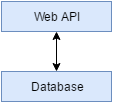
\includegraphics[width=0.60\textwidth]{images/database_layer}
 \caption{Example subsystem description diagram}
\end{figure}

\subsection{Web API}
The Web API allows access of data for clients

\subsubsection{Assumptions}
The Web API makes an assumption that bad calls will be ignored and security will not be needed.

\subsubsection{Responsibilities}
Web API should parse the html request.

\subsubsection{Subsystem Interfaces}

\begin {table}[H]
\caption {Subsystem interfaces} 
\begin{center}
    \begin{tabular}{ | p{1cm} | p{6cm} | p{3cm} | p{3cm} |}
    \hline
    ID & Description & Inputs & Outputs \\ \hline
    \#01 & HTML Interface & \pbox{3cm}{HTML Requests} & \pbox{3cm}{JSON Objects}  \\ \hline
    \#02 & Database Interface & \pbox{3cm}{JSON Objects} & \pbox{3cm}{JSON Objects}  \\ \hline
    \end{tabular}
\end{center}
\end{table}

\subsection{Database}
The Database provides routes to all data and stores the final data that is ready to be fetched by other layers.

\subsubsection{Assumptions}
The Database should only store valid data and ignore invalid data.

\subsubsection{Responsibilities}
The Database should store data and keep it ready to deliver to requesters.

\subsubsection{Subsystem Interfaces}
The database itself does not have any system interfaces.
\newpage
\section{Web Service Layer Subsystems}
This layer allows access for data web based clients. Clients connect to the gateway to request resources. If the request passes the authentication, it will be sent to the core.

\begin{figure}[h!]
	\centering
 	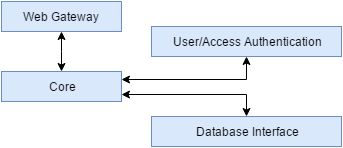
\includegraphics[width=0.60\textwidth]{images/web_service_layer}
 \caption{Example subsystem description diagram}
\end{figure}

\subsection{Web Gateway}
Web Gateway is a html controller that parses the html request.

\subsubsection{Assumptions}
The Web Gateway subsystem makes the assumption that any improperly formatted html request will be ignored.

\subsubsection{Responsibilities}
Web Gateway should parse the html request.

\subsubsection{Subsystem Interfaces}

\begin {table}[H]
\caption {Subsystem interfaces} 
\begin{center}
    \begin{tabular}{ | p{1cm} | p{6cm} | p{3cm} | p{3cm} |}
    \hline
    ID & Description & Inputs & Outputs \\ \hline
    \#01 & HTML Interface & \pbox{3cm}{HTML Requests} & \pbox{3cm}{JSON Objects}  \\ \hline
    \#02 & Database Interface & \pbox{3cm}{JSON Objects} & \pbox{3cm}{JSON Objects}  \\ \hline
    \end{tabular}
\end{center}
\end{table}

\subsection{User/Access Authentication}
User/Access Authentication validates the html request based on the tokens.

\subsubsection{Assumptions}
The User/Access Authentication subsystem makes the assumption that any unauthorized html tokens will be ignored.

\subsubsection{Responsibilities}
User/Access Authentication should check the html request for its validity. 

\subsubsection{Subsystem Interfaces}

\begin {table}[H]
\caption {Subsystem interfaces} 
\begin{center}
    \begin{tabular}{ | p{1cm} | p{6cm} | p{3cm} | p{3cm} |}
    \hline
    ID & Description & Inputs & Outputs \\ \hline
    \#01 & HTML Interface & \pbox{3cm}{HTML Requests} & \pbox{3cm}{JSON Objects}  \\ \hline
    \#02 & Database Interface & \pbox{3cm}{JSON Objects} & \pbox{3cm}{JSON Objects}  \\ \hline
    \end{tabular}
\end{center}
\end{table}

\subsection{Database Interface}
Database Interface helps connect the core to the actual database to fetch and store the data in the actual database.

\subsubsection{Assumptions}
The database Interface subsystem makes the assumption that the data passing through it is in the final form so that it can be stored in the actual database.

\subsubsection{Responsibilities}
The database Interface should allow the data to pass to the Database Layer. Invalid data should be buffered within the subsystem before passing it to the Database Layer.

\subsubsection{Subsystem Interfaces}

\begin {table}[H]
\caption {Subsystem interfaces} 
\begin{center}
    \begin{tabular}{ | p{1cm} | p{6cm} | p{3cm} | p{3cm} |}
    \hline
    ID & Description & Inputs & Outputs \\ \hline
    \#01 & Database Interface & \pbox{3cm}{JSON Objects} & \pbox{3cm}{JSON Objects}  \\ \hline
    \end{tabular}
\end{center}
\end{table}

\subsection{Core}
The Web Service Layer Core subsystem will distribute all the parsed html requests to the appropriate layer in the total system.

\subsubsection{Assumptions}
Core subsystem makes the assumption that there would be some subsystem that would take care of the distributed parsed requests.

\subsubsection{Responsibilities}
The core subsystem should make sure to distribute the parsed html requests to the appropriate subsystem.

\subsubsection{Subsystem Interfaces}

\begin {table}[H]
\caption {Subsystem interfaces} 
\begin{center}
    \begin{tabular}{ | p{1cm} | p{6cm} | p{3cm} | p{3cm} |}
    \hline
    ID & Description & Inputs & Outputs \\ \hline
    \#01 & HTML Interface & \pbox{3cm}{HTML Requests} & \pbox{3cm}{JSON Objects}  \\ \hline
    \#02 & Database Interface & \pbox{3cm}{JSON Objects} & \pbox{3cm}{JSON Objects}  \\ \hline
    \end{tabular}
\end{center}
\end{table}
\newpage
\section{Web Client Layer Subsystems}
A browser interface that allows the user to interact with the entire system.

\begin{figure}[h!]
	\centering
 	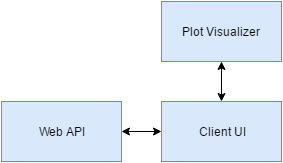
\includegraphics[width=0.60\textwidth]{images/web_client_layer}
 \caption{Example subsystem description diagram}
\end{figure}

\subsection{Web API}
The Web API makes calls to the web service layer. It also stores and provides user authentication credentials.

\subsubsection{Assumptions}
The Web API cannot assume the web service layer is always operating and will respond.

\subsubsection{Responsibilities}
It should maintain connection to web service layer. It should pass all requests from other subsystems. It should keep user authentication credentials so that API calls can be validated.

\subsubsection{Subsystem Interfaces}

\begin {table}[H]
\caption {Subsystem interfaces} 
\begin{center}
    \begin{tabular}{ | p{1cm} | p{6cm} | p{3cm} | p{3cm} |}
    \hline
    ID & Description & Inputs & Outputs \\ \hline
    \#01 & HTML Interface & \pbox{3cm}{HTML Requests} & \pbox{3cm}{JSON Objects}  \\ \hline
    \end{tabular}
\end{center}
\end{table}

\subsection{Plot Visualizer}
Take data and convert it into image. It should take the plot data and graph out the elements and generate a visual example.

\subsubsection{Assumptions}
The input data is valid.

\subsubsection{Responsibilities}
It should convert data to image and be able to generate visual example.

\subsubsection{Subsystem Interfaces}
\begin {table}[H]
\caption {Subsystem interfaces} 
\begin{center}
    \begin{tabular}{ | p{1cm} | p{6cm} | p{3cm} | p{3cm} |}
    \hline
    ID & Description & Inputs & Outputs \\ \hline
    \#01 & Plot data & \pbox{3cm}{JSON Object} & \pbox{3cm}{Image or JS Canvas}  \\ \hline
    \end{tabular}
\end{center}
\end{table}

\subsection{Client UI}
A JavaScript based UI to allow the user to see the status of the farmbot, send commands, and schedule various activities.

\subsubsection{Assumptions}
The client browser will run the needed JavaScript. Unsupported browsers will be notified and rejected.

\subsubsection{Responsibilities}
The Client UI should maintain minimal resource usage to maintain the expected functionality.

\subsubsection{Subsystem Interfaces}
\begin {table}[H]
\caption {Subsystem interfaces} 
\begin{center}
    \begin{tabular}{ | p{1cm} | p{6cm} | p{3cm} | p{3cm} |}
    \hline
    ID & Description & Inputs & Outputs \\ \hline
    \#01 & Javascript & \pbox{3cm}{User Interaction} & \pbox{3cm}{Web Page}  \\ \hline
    \end{tabular}
\end{center}
\end{table}
\newpage

%%% References
\bibliographystyle{plain}
\bibliographystyle{reference/IEEEtran_custom}
\bibliography{reference/refs}{}

\end{document}